%
% tikztemplate.tex -- template for standalon tikz images
%
% (c) 2021 Prof Dr Andreas Müller, OST Ostschweizer Fachhochschule
%
\documentclass[tikz]{standalone}
\usepackage{amsmath}
\usepackage{times}
\usepackage{txfonts}
\usepackage{pgfplots}
\usepackage{csvsimple}
\usepackage{mathrsfs}
\usetikzlibrary{arrows,intersections,math}
\begin{document}
\definecolor{darkgreen}{rgb}{0,0.6,0}
\def\skala{1}
\begin{tikzpicture}[>=latex,thick,scale=\skala]

%
% Koordinatengitter
%
\def\grid{
\node at (0,0) {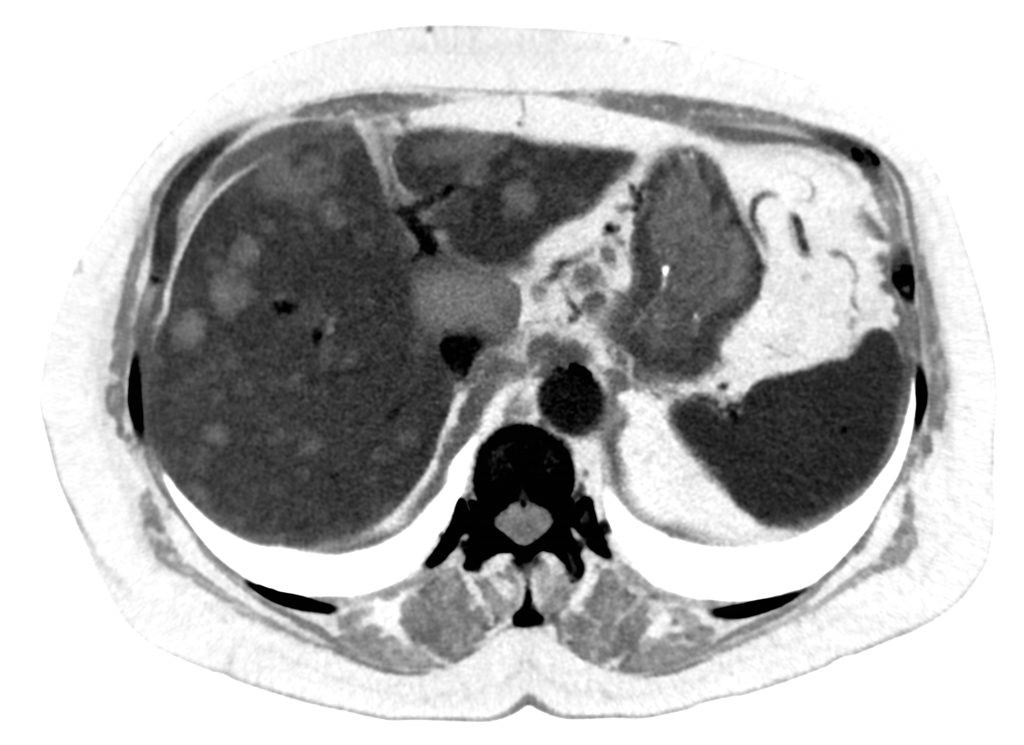
\includegraphics[width=2.5cm]{querschnitt.jpg}};
\node[color=white] at (-0.5,0.2) [scale=0.8] {$f(x,y)$};
\fill[color=white,opacity=0.5] (-1.5,-1.5) rectangle (1.5,1.5);
\draw[->] (-1.5,0) -- (1.5,0) coordinate[label={$x$}];
\draw[->] (0,-1.5) -- (0,1.5) coordinate[label={right:$y$}];
\draw[->,color=red] (1.2,1.3) to[out=20,in=160] (2,1.3);
\node[color=red] at (1.6,1.4) [above] {$\mathscr{F}$};
\begin{scope}[xshift=3.2cm]
\draw[->] (-1.5,0) -- (1.5,0) coordinate[label={$k$}];
\draw[->] (0,-1.5) -- (0,1.5) coordinate[label={right:$l$}];
\end{scope}
}

%
% linkes bild
%
\def\blau#1{
	\foreach \y in {-1.2,-0.8,...,1.2}{
		\draw[color=#1] (-1.5,\y) -- (1.5,\y);
		\fill[color=#1] (3.2,\y) circle[radius=0.06];
	}
	\node[color=#1] at (-1.0,0.6) {$\vartheta_0=0\mathstrut$};
}

\begin{scope}[xshift=-3.5cm]
\grid
\blau{blue}
\node at (1.6,-1.6) {(a)\strut};
\end{scope}

\begin{scope}[xshift=3.5cm]
\grid
\blau{blue!40}
\def\w{60}
\foreach \y in {-1.6,-1.2,...,2.0}{
	\begin{scope}
		\clip (-1.5,-1.5) rectangle (1.5,1.5);
		\draw[color=darkgreen] ({\y*cos(\w)},{\y*sin(\w)})
			-- +({2*sin(\w)},{-2*cos(\w)});
		\draw[color=darkgreen] ({\y*cos(\w)},{\y*sin(\w)})
			-- +({-2*sin(\w)},{2*cos(\w)});
	\end{scope}
	\fill[color=darkgreen] ({3.2+\y*cos(\w)},{\y*sin(\w)})
		circle[radius=0.06];
	\node[color=darkgreen]
		at ({-1.5*cos(\w-90)-0.6*sin(\w-90)},{-1.5*sin(\w-90)+0.6*cos(\w-90)})
		[rotate={\w-90}] {$\vartheta=\vartheta_1$};
}
\node at (1.6,-1.6) {(b)\strut};
\end{scope}

\end{tikzpicture}
\end{document}

